% \usepackage{amsmath}

\begin{table}[h]
    \centering
    \begin{tabular}{ll}
        \toprule
        \textbf{Title} & Seq2sql: Generating structured queries from natural language \\
        & using reinforcement learning\\
        \midrule
        \textbf{Venue} & arXiv \\
        \textbf{Year}  & 2017 \\
        \textbf{URL}   & \url{https://arxiv.org/pdf/1709.00103.pdf} \\
        \bottomrule
    \end{tabular}
    \vspace{1em}
\end{table}

\paragraph{Background.}
NLI (Natural Language Interface) under the broader field of semantic parsing has been developed to enable people to interact with computers through natural languages. The authors of this paper focus on a specific area of NLI: translating the questions in natural language into SQL queries, so that the user can access the relational databases without knowing a query language. 

\paragraph{Summary of contributions.}
The contributions of the authors' work include two parts. First, they used the augmented pointer network, introduced the rewards from reinforcement learning into the loss function, and developed a deep sequence-to-sequence network, called Seq2SQL, which achieved a very good results on query generation. Second, they released a new dataset called WikiSQL, consisting of over 80,000 manually annotated instances of natural language questions with SQL queries for tables extracted from Wikipedia, together with a query execution engine for policy learning.

More details of their model are provided as follows:

For all models introduced in our lectures, the size of the output dictionary must be fixed before the training starts, and we usually build a large dictionary consisting all tokens we may possibly encounter. However, for the query problem, the output is expected to contain only column names from tables and words from inputs, plus all unique words in SQL commands, and therefore a more efficient way is to use a Augmented Pointer Network which generates the SQL query simply by selecting from an input sequence token-by-token, instead of defining a huge output library. The authors defined the input to their model as
\begin{align*}
    x = \Big[\langle {\rm col} \rangle; x_1^{\rm c};x_2^{\rm c};...;x_N^{\rm c};\langle {\rm sql} \rangle; x^{\rm s}; \langle {\rm question} \rangle; x^{\rm q} \Big]
\end{align*}
by concatenating all column names $x_1^{\rm c}, x_2^{\rm c},...,x_N^{\rm c}$, with all unique words in SQL commands $x^{\rm s}$ and the sequence of words in the input $x^{\rm q}$. 

% Selecting the token during output has been achieved using the attention technique we learned from lectures. The scalar attention score was calculated as
% \begin{align*}
%     \alpha^{\rm ptr}_{s,t} = W^{\rm ptr} \tanh \left( U^{\rm ptr} g_t + V^{\rm ptr} h_t \right)
% \end{align*}
% at the output step $s$ for each position $t$ in the input. The $g_s$ and $h_t$ are states of the decoder and encoder respectively, and the input token with the largest attention will be generated as the next token.

\begin{figure}[ht!]
    \centering
    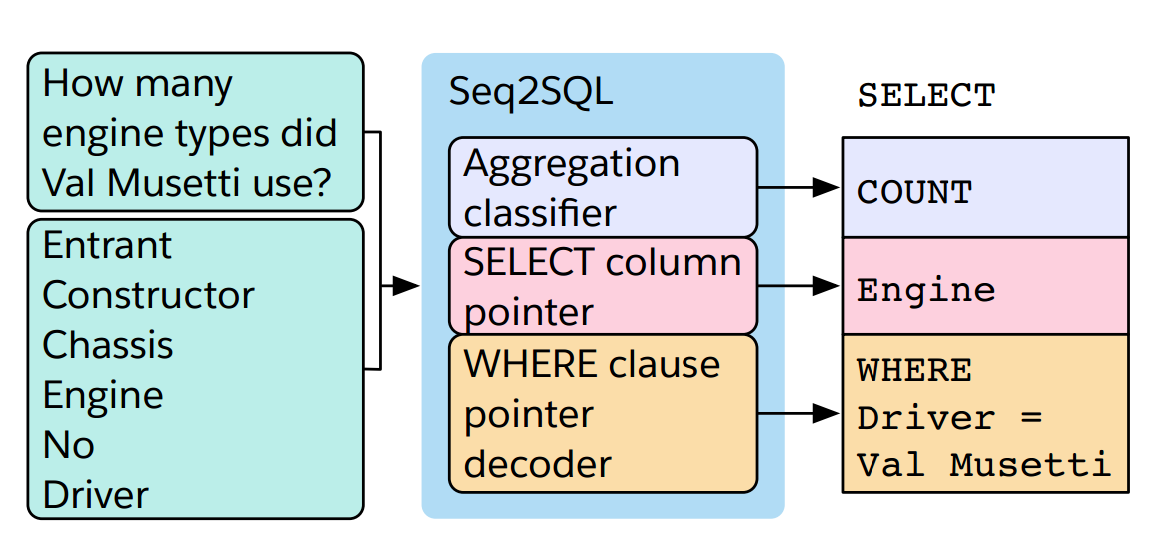
\includegraphics[width = 200px]{proposal/Seq2SQL_model.png} 
    \caption{The three components of the Seq2SQL model are responsible for generating the three parts of a SQL query. In the top left block is the question and in the bottom left block are column names. Figure from \cite{zhong2017seq2sql}.}
    \label{app1}
\end{figure}

Apart from the Augmented Pointer Network, the author also made full use of the structure of SQL command to build their Seq2SQL model. A SQL query consists of three components: an aggregation operator (can be NULL), the column(s), and a WHERE clause. And the model has three separate components to deal with them. For the aggregation operator and the column(s), the attention technique summarized before was used with the cross entropy loss. The interesting part is how the authors use the Reinforcement Learning to supervise the generation of WHERE clause.

The special thing about the WHERE clause is that the order may not matter. For example \textbf{SELECT name FROM insurance WHERE age > 18 AND gender = "male"} and \textbf{SELECT name FROM insurance WHERE gender = "male" AND age > 18} are equivalent, but using cross entropy may wrongly penalize one of them. To handle this, the loss function is computed as the negative expected reward over possible WHERE clauses by executing the generated WHERE clause $q(y)$ together with the ground truth $q_g$ against the database and compared the results . The reward $R(q(y), q_g)$ is 1 if $q(y)$ is not a valid WHERE clause, -1 if $q(y)$ is a valid WHERE clause and executes to an incorrect result, and +1 if it executes to the correct result. The loss function of the where clause $L^{\rm whe} = - \mathbb{E}_y\left[ R(q(y), q_g) \right]$, and the gradient is calculated as
\begin{align*}
    \nabla L^{\rm whe}_{\Theta} & = -\nabla_{\Theta} \left(\mathbb{E}_{y \sim p_y}\left[ R(q(y), q_g) \right]   \right) \\
    &= - \mathbb{E}_{y \sim p_y}\left[ R(q(y), q_g)  \nabla_{\Theta} \sum_t(\log p_y(y_t, \Theta)) \right] \\
    &\approx -R(q(y), q_g) \nabla_{\Theta} \sum_t(\log p_y(y_t, \Theta))
\end{align*}
where the expected gradient is approximated using a single Monte-Carlo sample $y$, and $p_y(y_t, \Theta)$ is the probability of choosing token $y_t$ during time step $t$. And the total loss $L = L^{\rm agg} + L^{\rm col} + L^{\rm whe}$. The author reported that Reinforcement Learning can generate higher quality WHERE clause that are ordered differently than ground truth.

\paragraph{Limitations and discussion.}
Despite the improvement the authors made, this paper still suffers from some limitations. First, although the inclusion of Reinforcement Learning helps to improve the model performance, such a performance is not significant. Without RL, the test accuracy was already 57.1\%, and RL only improved the accuracy by 2.3\%. Second, all the experiments were performed on the WikiSQL dataset developed by the authors. WikiSQL may not be representative of all databases, and therefore the results reported in the paper may not be strong enough. Finally, the questions input to the model are in simple forms. They always start with key words like "how many" and "what". A query like "show me the number of" or "find the" may not work. The interface built via this model is not user-friendly enough.

\paragraph{Why this paper?}
In a curious fashion this paper addresses the translation from a natural human language to an intentionally designed, structured, and context-free language used by computers, and it is highly cited (by 512). Because we are translating from a large domain to a very narrow subset of human expression, this problem benefits from the added structure and rigidity of the target language.

\paragraph{Wider research context.}
 In general, tasks like this help us translate from natural language to context free grammars, which are widely used in programming languages and interfaces. However, as with natural languages, even context free grammars allow nested structures and permuted orders \cite{zeng2020recparser, allamanis2018survey}. This poses difficulties for RNNs and even LSTMs due the problem of memory selection, i.e. did I already output that WHERE clause? Ultimately, it would be nice to develop enormous encoder-decoder frameworks similar to those used by Google Translate to encode natural language human computer tasks and decode them into a variety of different execution languages, whether that be bash, zsh, nushell, or a programming language like python or rust. This field is interesting in the wider context because it broaches the communication gap between humans and computers.